% $Id: template.tex 11 2007-04-03 22:25:53Z jpeltier $

\documentclass{vgtc}                          % final (conference style)
%\documentclass[review]{vgtc}                 % review
%\documentclass[widereview]{vgtc}             % wide-spaced review
%\documentclass[preprint]{vgtc}               % preprint
%\documentclass[electronic]{vgtc}             % electronic version

%% Uncomment one of the lines above depending on where your paper is
%% in the conference process. ``review'' and ``widereview'' are for review
%% submission, ``preprint'' is for pre-publication, and the final version
%% doesn't use a specific qualifier. Further, ``electronic'' includes
%% hyperreferences for more convenient online viewing.

%% Please use one of the ``review'' options in combination with the
%% assigned online id (see below) ONLY if your paper uses a double blind
%% review process. Some conferences, like IEEE Vis and InfoVis, have NOT
%% in the past.

%% Figures should be in CMYK or Grey scale format, otherwise, colour 
%% shifting may occur during the printing process.

%% These few lines make a distinction between latex and pdflatex calls and they
%% bring in essential packages for graphics and font handling.
%% Note that due to the \DeclareGraphicsExtensions{} call it is no longer necessary
%% to provide the the path and extension of a graphics file:
%% \includegraphics{diamondrule} is completely sufficient.
%%
\ifpdf%                                % if we use pdflatex
  \pdfoutput=1\relax                   % create PDFs from pdfLaTeX
  \pdfcompresslevel=9                  % PDF Compression
  \pdfoptionpdfminorversion=7          % create PDF 1.7
  \ExecuteOptions{pdftex}
  \usepackage{graphicx}                % allow us to embed graphics files
  \DeclareGraphicsExtensions{.pdf,.png,.jpg,.jpeg} % for pdflatex we expect .pdf, .png, or .jpg files
\else%                                 % else we use pure latex
  \ExecuteOptions{dvips}
  \usepackage{graphicx}                % allow us to embed graphics files
  \DeclareGraphicsExtensions{.eps}     % for pure latex we expect eps files
\fi%

% \usepackage{natbib}


%% it is recomended to use ``\autoref{sec:bla}'' instead of ``Fig.~\ref{sec:bla}''
\graphicspath{{figures/}{pictures/}{images/}{./}} % where to search for the images

\usepackage{microtype}                 % use micro-typography (slightly more compact, better to read)
\PassOptionsToPackage{warn}{textcomp}  % to address font issues with \textrightarrow
\usepackage{textcomp}                  % use better special symbols
\usepackage{mathptmx}                  % use matching math font
\usepackage{times}                     % we use Times as the main font
\renewcommand*\ttdefault{txtt}         % a nicer typewriter font
\usepackage{cite}                      % needed to automatically sort the references
\usepackage{tabu}                      % only used for the table example
\usepackage{booktabs}                  % only used for the table example
%% We encourage the use of mathptmx for consistent usage of times font
%% throughout the proceedings. However, if you encounter conflicts
%% with other math-related packages, you may want to disable it.


%% If you are submitting a paper to a conference for review with a double
%% blind reviewing process, please replace the value ``0'' below with your
%% OnlineID. Otherwise, you may safely leave it at ``0''.
\onlineid{0}

%% declare the category of your paper, only shown in review mode
\vgtccategory{Research}

%% allow for this line if you want the electronic option to work properly
\vgtcinsertpkg

%% In preprint mode you may define your own headline.
%\preprinttext{To appear in an IEEE VGTC sponsored conference.}

%% Paper title.

\title{Future of Work Final Report}

%% This is how authors are specified in the conference style

%% Author and Affiliation (single author).
%%\author{Roy G. Biv\thanks{e-mail: roy.g.biv@aol.com}}
%%\affiliation{\scriptsize Allied Widgets Research}

%% Author and Affiliation (multiple authors with single affiliations).
%%\author{Roy G. Biv\thanks{e-mail: roy.g.biv@aol.com} %
%%\and Ed Grimley\thanks{e-mail:ed.grimley@aol.com} %
%%\and Martha Stewart\thanks{e-mail:martha.stewart@marthastewart.com}}
%%\affiliation{\scriptsize Martha Stewart Enterprises \\ Microsoft Research}

%% Author and Affiliation (multiple authors with multiple affiliations)
\author{Ethan J. Holen\thanks{e-mail: eholen@rams.colostate.edu}\\ %
        \scriptsize Colorado State University %
}

%% A teaser figure can be included as follows, but is not recommended since
%% the space is now taken up by a full width abstract.
%\teaser{
%  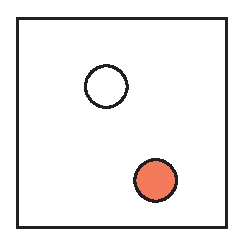
\includegraphics[width=1.5in]{sample.eps}
%  \caption{Lookit! Lookit!}
%}


%% ACM Computing Classification System (CCS). 
%% See <http://www.acm.org/class/1998/> for details.
%% The ``\CCScat'' command takes four arguments.

% \CCScatlist{ 
%   \CCScat{K.6.1}{Management of Computing and Information Systems}%
% {Project and People Management}{Life Cycle};
%   \CCScat{K.7.m}{The Computing Profession}{Miscellaneous}{Ethics}
% }

%% Copyright space is enabled by default as required by guidelines.
%% It is disabled by the 'review' option or via the following command:
% \nocopyrightspace

%%%%%%%%%%%%%%%%%%%%%%%%%%%%%%%%%%%%%%%%%%%%%%%%%%%%%%%%%%%%%%%%
%%%%%%%%%%%%%%%%%%%%%% START OF THE PAPER %%%%%%%%%%%%%%%%%%%%%%
%%%%%%%%%%%%%%%%%%%%%%%%%%%%%%%%%%%%%%%%%%%%%%%%%%%%%%%%%%%%%%%%%

\begin{document}

%% The ``\maketitle'' command must be the first command after the
%% ``\begin{document}'' command. It prepares and prints the title block.

%% the only exception to this rule is the \firstsection command
\firstsection{Introduction}




\maketitle

%% \section{Introduction} %for journal use above \firstsection{..} instead

With augmented reality (AR) devices becoming cheaper and more common in the home and workplace, the range of potential uses for it in everyday life has expanded. One of the areas which AR can now assist in is aiding in physical construction or assembly tasks. Previously users have had to read instructions or watch videos to learn how to put together a new piece of furniture or appliance. This can be challenging especially when working with small or fragile components, and can prove expensive if pieces are broken. Along with the mental cost of context switching between the video or tutorial and the task at hand. With the ever increasing availability of AR, the potential for virtual tutorials in which a user could go step by step through the building process virtually are now available. This experiment seeks to examine ways in which instructions in AR could improve upon the current instruction types.

This can now potentially include helping with daily tasks such as tutorials to help with building physical object such as furniture or new appliances. Instead of the user watching a video on their smartphone and building the object at the same time, they could now have the opportunity to be guided through the process with a digital overlay of the task in AR. This style of tutorial could minimize context switching, helping to minimize errors and maximize speed in completing simple at home construction projects.

The purpose of this experiment is to explore the benefits of different instruction types within an AR environment.


\section{Related Work}

Research into the field of AR tutorials and building instructions has been an ongoing field of research for a considerable amount of time. Beginning in 1992 with Caudell and Miezell \cite{Caudell92} presented a head mounted display which could show positions and textual queues for a drilling task. This research spurred a significant number of new possibilities for research into how building tasks could be improved with this new augmented reality model.

The work done in these papers has sparked significant interest in using AR as a tool to teach new skills, especially in assembly tasks. These techniques have so far been used and tested in industrial and military applications in which the environment is specifically tailored for this particular construction task. 

Columbia University published a paper on this subject called "Evaluating the Benefits of Augmented Reality for Task Localization in Maintenance of an Armored Personnel Carrier Turret" which focused on the application of AR in supporting armored vehicle mechanics \cite{Henderson09}. This experiment was "designed to facilitate task comprehension,location, and execution" \cite{Henderson09} of the expert tank mechanics who would usually be performing these repairs. This study found that the AR system improved on the time and head movement between tasks in the sequence.

Another recently published paper called "Comparing Conventional and Augmented Reality Instructions for Manual Assembly Tasks" explored the benefits of using AR over other instruction types \cite{Blattgerste17}. This experiment compared different instruction types namely AR on phone and headset as well as standard paper instructions and analyzed their results. This study found that participants completed the basic building tasks faster with the standard paper instructions but made the fewest errors when using the Hololens AR headset. 

More general studies have been completed having to do with different instruction types and their benefits. In 2019 IEEE had a paper called "Annotation vs. Virtual Tutor: Comparative Analysis on the Effectiveness of Visual Instructions in Immersive Virtual Reality" \cite{Lee19}. This paper compared the differences between a written instruction and an instruction acted out by a virtual tutor in a VR environment. This study found that the group with written instructions had both better recall of the task and where able to complete the task faster than the group with a virtual tutor \cite{Lee19}. These results could potentially be used in this experiment to determine one of the instruction types as being a written set of instructions.

Another important paper was written by the university of Stuttgart in Germany which explored the usage of AR instructions in an industrial environment over an extended period of time \cite{Funk17}. This experiment was conducted over 11 days and compared expert and untrained users in the environment. This study found that there was a decrease in performance for participants who were already experts at the task, but a significant improvement in untrained worker performance. \cite{Funk17}

These studies highlight some of the interesting and important questions that can be asked about the usage of AR for various building tasks. The also highlight some of the ways in which this method of instruction has been found not to work. Given that our participants are not experts in the task which they will be performing at least one of our instruction methods should see some improvement in task completion time or accuracy over the different building tasks.

\begin{figure}[!htbp]
    \centering
    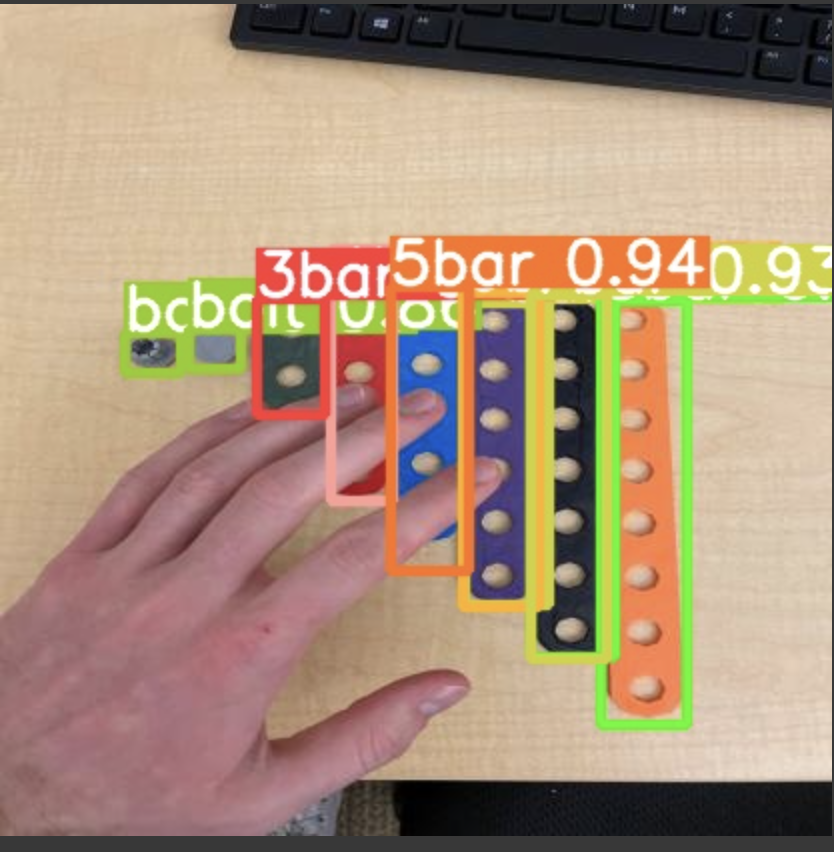
\includegraphics[width=\columnwidth]{bars-identified.png}
    \caption{3D Printed bars and bolt identified with tensorflow machine learning model.}
    \label{fig:bars_idd}
\end{figure}


\nocite{Ros20}


\section{Methodology}


This experiment will follow a between subjects design. The independent variable will be the type of instruction the participant is randomly assigned, and the dependent variables will be the speed and the accuracy with which they complete each task.


\subsection{Apparatus}





The environment for this experiment will be a combination of virtual and physical interfaces for the user. The virtual environment will be provided by the Hololens 2 augmented reality headset by Microsoft, combined with the Oak-D machine learning camera form open-CV. The bars will be identified with a tensorflow machine learning model as pictured in \autoref{fig:bars_idd} The virtual environment will be provided by an application built with the mixed reality toolkit. 

\begin{figure}[!htbp]
    \centering
    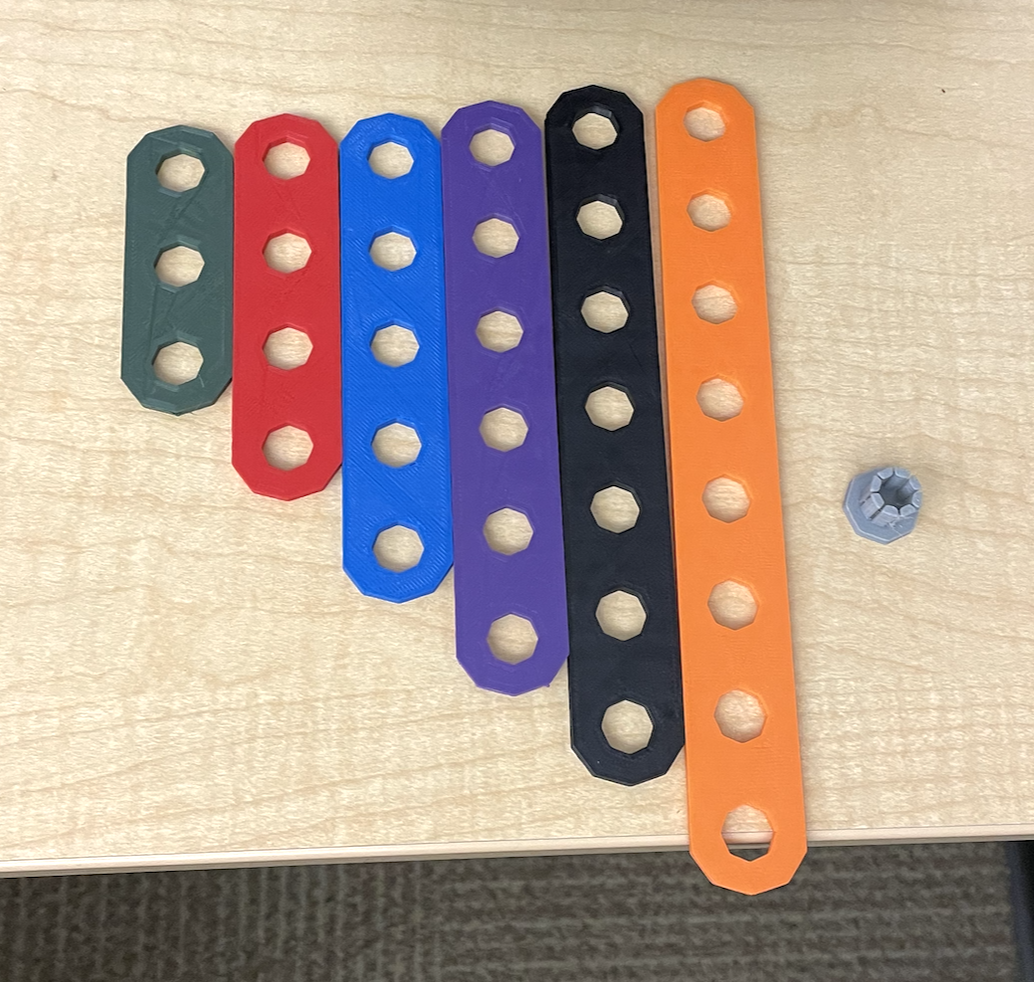
\includegraphics[width=\columnwidth]{bars.png}
    \caption{3D Printed bars and bolt from size three to size eight.}
    \label{fig:bars}
\end{figure}


The physical interface of the experiment consists of a series of 3D printed bars and bolts which will constitute the construction materials for the building task. These will each have a unique color to help with the machine learning model which can be seen in \autoref{fig:bars} Each building task will be defined by a different shape that will need to be built by the participant, using the provided bars and bolts. Proper Completion of this task will be determined by the Oak-D cameras machine learning model. 




\subsection{Modified Apparatus (for usability study)}

*(This experiment had to be limited from its previous version to a usability study described below)

The Apparatus will be mostly the same as described in the Apparatus subsection above, with the exception of the Hololens 2 augmented reality headset. Regretfully, development of the machine learning model took the majority of the allotted time for the development of this experiment and I was only able to get a basic usability study in place by the time that I needed to start running experiments. The modified apparatus consisted of a monitor which displayed both instructions for building the given shape along side the bar identification software displayed through the oak-d camera. Using these two guides the user built the shape using the provided 3D printed bars.



\subsection{Procedure}



Each participant will be asked to sit at the desk and walked through how to put on and adjust the Hololens. The participant will then be guided through a basic tutorial detailing the proper use of the augmented reality environment along with a basic building tutorial. Before the tutorial the participant will be randomly assigned to one of the instruction groups. The participant will then be guided through each of the building tasks with their specific assigned instruction set. After the completion of the experiment the participant will be asked for any feedback they might have in a small questionnaire and then dismissed.



\subsection{Modified procedure (for usability study)}

*(This experiment had to be limited from its previous version to a usability study described below)

Each participant will be asked to sit at the desk and guided through the directions for building a shape using the 3d printed Meccano bars. They will then be presented with instructions to build the specific shape for the experiment along with the bar visualization software. These instructions will not be color coded like the bars are, forcing the user to count the holes in each bar on the diagram and hopefully causing them to use the software more than they otherwise would to help with identifying the bars that they are using. Using the software and the picture instructions the participant will be asked to complete the building task. The participant will also be informed that using the bar identification software is optional, and that they are free to use it as needed. After task completion they will be asked to fill out the usability study to determine their experience in using the software. As well as to gather their general sentiment on what parts of the software might need improvement and if there where any areas of general irritation with it.







\section{Results}

The following section will be a discussion of the results collected from the google form that participants where asked to fill out after completing the usability study. By the end of this experiment ten participants were able to participate in the experiment and fill out the google form. The form itself consisted of nine total questions pertaining to different components of the users experience of the software. In the following questions the machine learning software written for this study which was presented to the user via a camera view on the monitor will be referred to as the "bar identification software". Each participant was made aware of this vernacular before beginning the experiment, as well as being told only to use the software if they found that it aided in the building task.



\subsection{Software Usage}

\begin{figure}[!htbp]
    \centering
    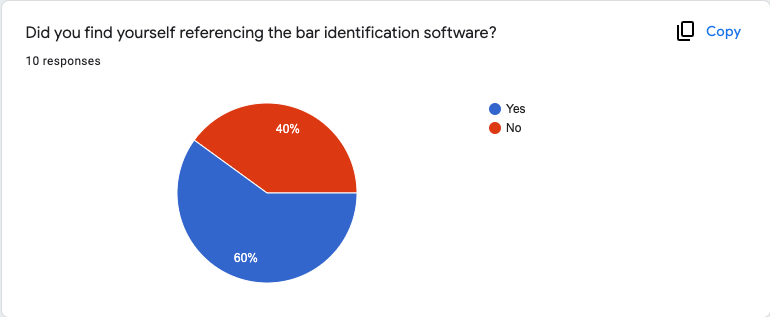
\includegraphics[width=\columnwidth]{pictures/usage1.png}
    \caption{Percentage of participants referencing the bar identification software}
    \label{fig:usage1}
\end{figure}


The first two questions in the survey pertain to the overall usage of the bar identification software. The first question in the survey seeks to ascertain how many participants actually used the software during the course of the experiment. As can be see in \autoref{fig:usage1} forty percent of the participants completely ignored the software and did not use it, while sixty percent did use the software to some degree. 

The chart in \autoref{fig:usage2} helps to further understand the overall usage of the software by each participant. The breakdown being that forty percent used the identification software roughly six to ten times while while sixty percent used the software zero to five times. In retrospect this question should have had an added zero category and then a one to five category to help with removing the percentage of people who did not use the bar identification software at all. Using the previous question to weed out the forty percent we can figure out that the new breakdown is: zero uses = 40 percent, 1-5 uses = 20 percent and 6-10 uses = 40 percent.



\begin{figure}[!htbp]
    \centering
    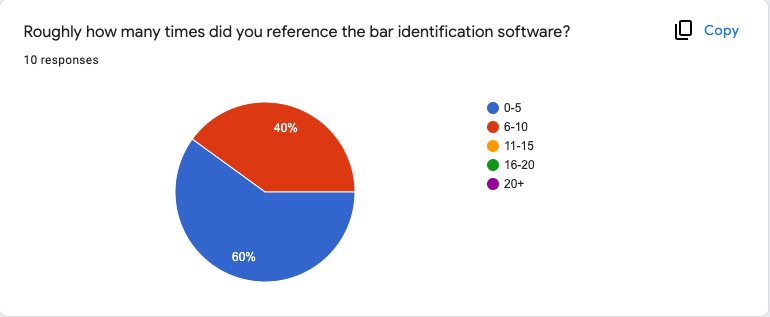
\includegraphics[width=\columnwidth]{pictures/usage2.png}
    \caption{Number of uses of the bar identification software}
    \label{fig:usage2}
\end{figure}

\subsection{User Experience}


The next question in the survey, displayed in \autoref{fig:helpful} asked the participant to rate their experience of using the software on a scale from 1-5. This rating system showed fifty percent of the participants giving a score of three out of five, while ten percent gave higher scores and forty percent gave lower scores of one and two. 





\begin{figure}[!htbp]
    \centering
    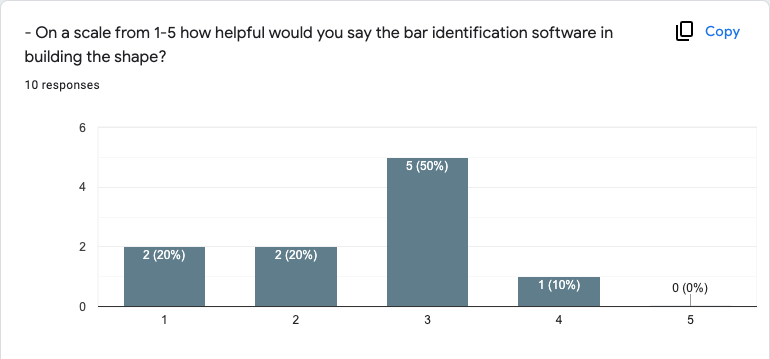
\includegraphics[width=\columnwidth]{pictures/helpful.png}
    \caption{Helpfulness of the software as rated by user 1-5}
    \label{fig:helpful}
\end{figure}


\subsection{Participant Feedback and Frustrations}

The remaining questions where long answer style and do not present any numerical data and will be discussed at length in the discussion section of the paper.


\section{Discussion}

Overall, the usage of the software was significantly higher than initially anticipated. In designing the usability study I considered requiring each participant to use the bar identification software in some way but then decided against it as it might skew the data in favor of the software. In making usage optional the data can now give a better idea of how participants may have used this software if it was presented to them in a real life building context, such as building IKEA furniture. 

The collected data shows that sixty percent of users will use the software if it is made available to them. Furthermore, around 40 percent of the participants who did use the software reported using it 6-10 times as a reference for their building task. This indicates a high level of participant interaction when 

\subsection{Participant Feedback and Frustrations}


The second half of google form asked participants various open ended questions pertaining to their usage of the software. In this section i will be discussing a summary of the answers which participants gave along with some of the inspirations for further project development which these answers encouraged. 

The first question asked of each participant was "In what situation could you see yourself using a system like this for a building task?". The most common response to this question was something along the lines of a basic building task such as a home construction project such as building furniture or a building toy like Lego's. One of the most interesting responses received from a participant was to use the software as a cooking aid in putting together a recipe. While this would be a rather difficult application to create for a general purpose kitchen, I could see how this might be valuable asset for new chefs trying to find their way around a complex restaurant kitchen which could be diagrammed out in advance. This software could then highlight in a kitchen or pantry where the next needed ingredient was stored and guide the cook to it. A large chain might find software like this beneficial in training their new cooks and giving them a familiarity with the kitchen.

The second question in the survey asked each participant, "How would you describe your overall experience with the software?". In retrospect this may have been too open ended of a question and led many of the participants to answer with NA or simply "Good" which was not the summary which I expected. Some participants noted that the software was difficult to see, which is understandable as the camera view which displayed the oak-d feed was very small. This will be modified in future experiments with this software as it may limit the usability and visibility especially to people who are visually impaired in some way. Another comment received was that the camera seemed delayed. This is likely because the oak-d could only achieve a frame rate of 22 with the image resolution of the training model. While this did not seem to bother many of the users, it is a bug which i would like to fix in future iterations of this experiment.

Questions three and four are linked in asking what the participants liked most and least about the experience of using the bar identification software. The most common praise of the software was that it helped the users to count how many holes where in the bar before they could have counted themselves. This was one of the most important achievements of the software in retrospect. While choosing the bar with the correct number of holes may seem to be a minor problem in this particular scenario one can easily see where this could prove extremely useful in other situations. For example in piece of IKEA furniture where all of the pieces get mixed up and it becomes difficult to tell one bolt from another. Or more importantly a surgeon accidentally choosing one medical instrument for a procedure when he meant to choose another. This feedback helps to reinforce that a bar identification software which has been retrofitted to other cases could be an extremely useful tool in quickly identifying visually identical objects in various scenarios. The negative feedback from the question "What did you like the least?" revolved mostly around any of the inaccurate guessed that the software made in identifying the bars. This was mostly due to the experiment being in a light which the training model did not like. I plan to remedy this in the next iteration by using more low light images in the training and testing data. The main confusion was between the dark purple 6 bar and the black 7 bar. Another issue was that the camera being to the right of the participant as this did not match up with their perspective, some mental rotation was required. This issue will hopefully be resolved in the next iteration of the experiment as the camera will be mounted on a headset, making the perspectives align almost perfectly.

The final question of the survey was "What, if anything, caused you frustration?". This was similar to the previous question about what the participant liked the least but I felt that it was worth asking to encourage the participants to find at leas two things which may have hindered their use of the software. In spite of this many of the frustrations are the same as the things which they liked least. The one statement which did stand out was that it was difficult to get the shape into position in the end. Some of the users had some difficulty in getting the software to identify the correct shape at the end. This is a portion of the experiment which I would generally like to improve upon as it is giving a lot of false positives.



\section{Conclusion}


In moving forward with this experiments development there are quite a few new avenues which this usability study has forced me to consider. Both because of user feedback and my own observations in watching the users interactions with the software and 3D printed bars.

Firstly in considering the instructions used to show the user how to build the bar. In future experiments I would like to add a more detailed step by step instruction rather than the current finished shape. Something similar to an IKEA furniture building guide so that the experiment becomes a more accurate test of that type of scenario. Though i would not change the black and white coloring of the instructions as it does add to the difficulty of building the shape. As well as adding to the realistic aspect of the experiment as most instructions are printed in black and white to limit costs of production.

Other improvements which could be made to the software include improving the machine learning model in various ways. Firstly in its performance in different lighting conditions, as the black and purple bars where occasionally confused during the study. The application itself which presents the camera view to the user could also be improved mainly in its sizing and frame rate. It may be difficult to improve both of these simultaneously since the smaller the image size used the higher the frame rate can be.

Overall I believe the results of this usability study will significantly aid in the construction of future experiments with this project It has also helped in highlighting errors and modifications which will need to be made in the future for this to become a viable experiment.















%\bibliographystyle{abbrv}
\bibliographystyle{abbrv-doi}
% \bibliographystyle{abbrv-doi-narrow}
%\bibliographystyle{abbrv-doi-hyperref}
%\bibliographystyle{abbrv-doi-hyperref-narrow}

\bibliography{FOW}
\end{document}
